\section{Reachable Workspace and Path Planning}
\label{sec:trajectory}

Following the developement of the limb's kinematic model, the next logical step is to verify the correctness of
the design and its behaviour through digital simulation. However, two preliminary steps are essential: the reachable
workspace of the system must be analyzed to understand its operational boundaries and a desired trajectory for the
end-effector must be designed.


\subsection{Workspace Definition and Analysis}

The reachable workspace of a manipulator is formally defined as the complete set of all Cartesian positions
$p = [x,y,z]^{T}$ that its end-effector can attain, given the physical constraints of its kinematic
chain \cite{ding2010locomotion}. It represents the entire volume of space accessible to the robot's
end-effector. For this 3-DOF limb, the workspace is determined by the three link lengths ($a_{1},a_{2},a_{3}$)
and, most critically, by the actuation limits imposed on its three joints ($q_{1},q_{2},q_{3}$).

To characterize this 3D volume, a two-stage approach is taken. First, the 2D planar workspace is analyzed.
This is done by fixing the Hip Joint at a neutral angle (e.g. $q_1 = \ang{0}$) and generating the boundary of
the leg's reach in a single vertical plane. A 2D cross-section is then obtained by sweeping the Knee
($q_2$) and Ankle ($q_3$) joints through their entire operational ranges. The resulting surface (Figure
\ref{fig:workspace_analysis}) is finally revolved around the Hip joint axis by sweeping $q_1$ through its own
range, thereby generating the final 3D reachable volume.

\begin{figure}[htbp]
    \centering
    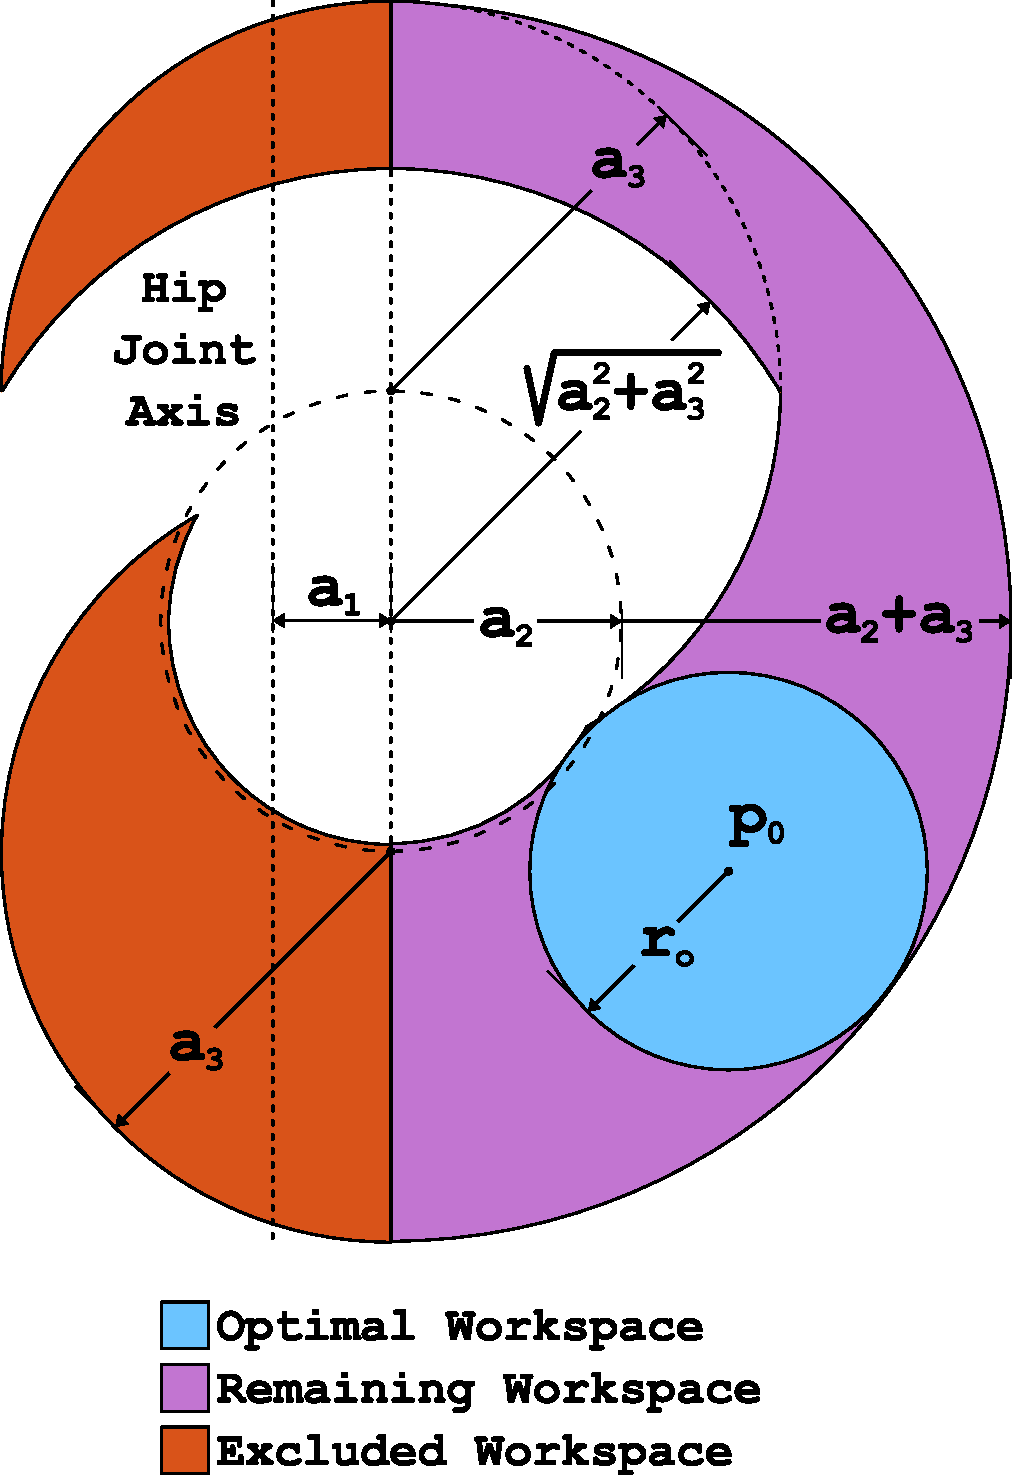
\includegraphics[width=0.7\textwidth]{images/workspace.pdf}
    \caption{Reachable Workspace Section for $q_1 = 0$}
    \label{fig:workspace_analysis}
\end{figure}

The actuator limits are the primary constraints defining this space. These limits are imposed both by the
physical components (i.e. the finite rotational range of the servo-motors) and by the mechanical design itself,
which is configured to prevent self-collision between links and other limbs.
For this specific implementation, the joint constraints are defined as follows:
\begin{equation*}
  q =[q_1, q_2, q_3]^T \in
  \left[-30^\circ, 30^\circ \right]
  \times
  \left[-90^\circ, 90^\circ \right]
  \times
  \left[30^\circ, 180^\circ \right]
\end{equation*}

As an additional safety measure, a portion of the resulting workspace (the red coloured area in Figure
\ref{fig:workspace_analysis}) is excluded from operation to prevent collisions with the robot's body or the mounting
structure. A simplified and safe \textbf{Optimal Work Region} is then defined by inscribing a sphere within the
remaining viable workspace depicted in blue. The center of this sphere, $p_0$, is designated as the leg's nominal
\textbf{Rest Position}, which will serve as the origin for gait trajectories.


\subsection{Trajectory Design}

Moving to trajectory generation, the goal is to create a function $p_d$ to define the motion of the foot.
The design of this trajectory is guided by several key principles and assumptions. Firstly, the path
must be parametric, dependent on both the desired walking speed $v$ and the direction of movement $\psi$.
Secondly, the trajectory primitive is generated relative to the leg's central rest position $p_0$, which is
eventually added as a final offset to determine the absolute path $p_d(t)$. For this initial derivation, we
also assume the ground is a flat, predictable plane at a constant height set to 0 (or $p_{z,0}$ after applying
the rest offset).

The gait cycle is composed of two distinct and well defined phases, which needs to be properly stitched together
to ensure smooth ($C^2$) motion. During the \textbf{Stance Phase}, the foot must remain stationary relative to
the ground as the body moves forward. This implies that the foot's velocity relative to the robot's body must
be constant and equal to $-v$ (along the $\psi$ direction). Consequently, the acceleration during this linear
phase is zero. Conversly, during the \textbf{Swing Phase}, the leg should relocate to start a new cycle
while also lifting off the ground.


\subsubsection{Quintic Polynomials}

The simplest and most widely adopted solution in robotics is using fifth-order (quintic) polynomials
\cite{biagiotti2008trajectory, siciliano2009robotics} to move between two points while matching boundary
conditions for position, velocity, and acceleration. A generic quintic polynomial is defined by six
coefficients ($c_0, \dots, c_5$):

$$ p(t) = c_5t^5 + c_4t^4 + c_3t^3 + c_2t^2 + c_1t + c_0 $$

The function $p(t)$ represents the position, while its first and second time derivatives, $v(t)$ and $a(t)$,
represent the velocity and acceleration, respectively:

$$ v(t) = \frac{dp}{dt} = 5c_5t^4 + 4c_4t^3 + 3c_3t^2 + 2c_2t + c_1 $$
$$ a(t) = \frac{d^2p}{dt^2} = 20c_5t^3 + 12c_4t^2 + 6c_3t + 2c_2 $$

To solve for the six unknown coefficients $\mathbf{c} = [c_0, c_1, c_2, c_3, c_4, c_5]^T$, we impose six
known boundary conditions, i.e. the desired position, velocity, and acceleration at the start time ($t = 0$)
and at the end time ($t = T$), where $T$ is the total duration of the movement. Then a system of six linear
equations can be derived and expressed in matrix form as $M \cdot \mathbf{c} = \mathbf{b}$:

$$
  \begin{bmatrix}
    1 & 0 & 0 & 0 & 0 & 0 \\
    0 & 1 & 0 & 0 & 0 & 0 \\
    0 & 0 & 2 & 0 & 0 & 0 \\
    1 & T & T^2 & T^3 & T^4 & T^5 \\
    0 & 1 & 2T & 3T^2 & 4T^3 & 5T^4 \\
    0 & 0 & 2 & 6T & 12T^2 & 20T^3
  \end{bmatrix}
  \begin{bmatrix}
    c_0 \\ c_1 \\ c_2 \\ c_3 \\ c_4 \\ c_5
  \end{bmatrix}
  =
  \begin{bmatrix}
    p_0 \\
    v_0 \\
    a_0 \\
    p_f \\
    v_f \\
    a_f
  \end{bmatrix}
$$

The vector of coefficients $\mathbf{c}$ can then be found by inverting the $6 \times 6$ matrix $M$ and
multiplying it by the vector of boundary conditions $\mathbf{b}$:

\begin{equation}
  \mathbf{c} = M^{-1} \cdot \mathbf{b}
  \label{eqn:quintic_poly_solution}
\end{equation}

The resulting coefficients are constants that depend only on the specified boundary conditions and the total
movement time $T$. The final trajectory $p(t)$ is then a continuous function of the generic time variable
$t \in [0, T]$.


\subsubsection{Horizontal Component}

We start by defining the 1D horizontal component of the trajectory, $p_h(t)$, as a function of normalized time
$t \in [0, 1]$, and representing the motion along the direction of travel $\psi$. The 2D path in the $XY$ plane
is simply this 1D motion projected onto the direction vector $\mathbf{d}(\psi) = [\sin(\psi), \cos(\psi)]^T$.

We define the \textbf{Duty Factor} $\beta$ as the fraction of the cycle spent in the Stance Phase (typically
$\beta > 0.5$ for structural stability, meaning that the robot is supported by at least 3 contact points at every
moment). This divides the normalized unit period into two segments:

$$ T_{stance} = \beta $$
$$ T_{swing} = (1-\beta) $$

The cycle is thus defined with the Swing Phase occurring for $t \in [0, T_{swing}]$ and the Stance Phase for
$t \in [T_{swing}, 1]$. The trajectory oscillates between a forward limit (touchdown) $p_1 = r$ and a backward
limit (liftoff) $p_2 = -r$. The total horizontal stroke is $S = 2r$.

During the Stance Phase, the motion is linear, connecting the touchdown point (at $t = T_{swing}$, $p = r$) to
the liftoff point (at $t = 1$, $p = -r$). The function $p_{h,stance}(t)$ is the equation of this line. Its slope,
the normalized velocity $v_{norm}$ is constant:

$$ v_{norm} = \frac{\Delta p}{\Delta t} = \frac{-2r}{\beta} $$
The trajectory for this phase and its derivatives are given by:
$$ p_{h,stance}(t) = p_1 + v_{norm} \cdot (t - T_{swing}) $$
$$ v_{h,stance}(t) = v_{norm} $$
$$ a_{h,stance}(t) = 0 $$
During the Swing Phase, we use the quintic polynomial method to move from the liftoff position back to the
touchdown position. This function must smoothly connect the end of the previous stance phase (at $t = 1$,
or $t = 0$ in the new cycle) to the start of the current stance phase (at $t = T_{swing}$).

To ensure $C^2$ continuity, we must match the position, velocity, and acceleration of the stance phase at both
ends. We solve for the polynomial $p_{h,swing}(t)$ over the interval $T = T_{swing}$ using the following
boundary conditions vector $\mathbf{b}_{h,swing} = [-r, v_{norm}, 0, r, v_{norm}, 0]^T$.
Solving Equation \ref{eqn:quintic_poly_solution} with this vector yields the specific coefficients for the
horizontal swing polynomial.


\subsubsection{Vertical Component}

Next, we define the vertical component of the motion, $p_z(t)$, relative to the ground plane.

During the stance phase the foot is on the ground providing propulsion, therefore $p_{z,stance}(t) = 0$. This
implies $v_{z,stance} = 0$ and $a_{z,stance}(t) = 0$.

During the swing phase, the leg must lift to a clearance height $H_{lift}$ ($= r$) and return to the ground.
This motion must also be $C^2$ continuous, connecting smoothly to the zero-motion of the Stance Phase. To
achieve this, the Swing Phase is split into two identical halves, "Lift-Up" and "Lift-Down", each with duration
$T_{lift} = T_{swing} / 2$.

We solve for the lift-up polynomial $p_{z,up}(t)$. The boundary conditions must match the stance phase at the
start ($t = 0$) and ensure a smooth apex at the peak ($t = T_{lift}$). The boundary conditions vector is
$\mathbf{b}_{z,up} = [0, 0, 0, H_{lift}, 0, 0]^T$. Then, the lift-down polynomial is a time-mirrored version of
the lift-up segment.

This two-stage approach guarantees $C^2$ continuity for the entire vertical trajectory: it starts from
$p=0, v=0, a=0$ (matching the stance end), achieves a smooth peak at $t = T_{lift}$, and returns to
$p=0, v=0, a=0$ at $t = T_{swing}$ (matching the stance start).


\subsubsection{Path Assembly}

The complete spatial geometry of the gait, $p_{prime}(t)$ is now fully designed, as a function of the
normalized time $t \in [0, 1]$. The complete primitive is assembled by combining the horizontal and vertical
components, projecting the horizontal motion onto the $X$ and $Y$ axes, and stitching the swing and stance
phases together:
$$
p_{prime}(t) =
  \begin{cases}
    \begin{bmatrix}
      p_{h,swing}(t) \sin(\psi) \\
      p_{h,swing}(t) \cos(\psi) \\
      p_{z,swing}(t)
    \end{bmatrix}
    & \text{Swing: } 0 \le t < T_{swing} \\
    \\
    \begin{bmatrix}
      p_{h,stance}(t) \sin(\psi) \\
      p_{h,stance}(t) \cos(\psi) \\
      0
    \end{bmatrix}
    & \text{Stance: } T_{swing} \le t \le 1 \\
  \end{cases}
$$
The desired path $p_d(t)$ sent to the controller is then obtained by biasing this primitive with the
leg's central rest position $p_d(t) = p_0 + p_{prime}(t)$.

Crucially, this formulation decouples the path's spatial geometry from its execution speed.
The function $p_{prime}(t)$ defines only the geometric path, with the input $t$ representing the percentage
of cycle completion, not the actual time.


\subsubsection{Walking Speed Dependance}

The desired physical walking speed $v$ is introduced by controlling how fast this normalized time $t$ advances
in the real world. This is achieved through a discrete-time implementation. First, we determine the required
real-time period ($T_{real}$) for one full gait cycle. The physical stroke $S = 2r$ must be covered at the
desired velocity $v$ during the stance phase, which lasts for a fraction $\beta$ of the total period, therefore
the total real-time period for the cycle is:
$$ T_{real} = \frac{2r}{\beta v} $$
In the control loop, the normalized path $p_{prime}(t)$ is discretized into $n$ samples (e.g. $n = 1000$).
A counter $k$ (where $0 \le k < n$) tracks the current step, and the corresponding normalized time is $t_k = k/n$.
The controller achieves the desired velocity $v$ by incrementing the counter $k$ at a specific real-time
frequency, $f$ determined by the real-time step $\Delta t_{real}$, which is the total period divided by the
number of samples:
$$ \Delta t_{real} = \frac{T_{real}}{n} = \frac{2r}{n \beta v} $$
The controller's update frequency is $f = 1 / \Delta t_{real}$. By adjusting this frequency $f$ (or its inverse,
the time step $\Delta t_{real}$), the desired velocity $v$ is precisely controlled, while the spatial trajectory
remains constant.